\documentclass{beamer}
\usetheme{Singapore}
\beamertemplatenavigationsymbolsempty
\begin{document}

    \title{NetVis}
    \subtitle{Network Security Visualisation Tool}
    \institute{
        James Nicholls, Dominik Peters, Albert Slawinski,\\
        Thomas Spoor, Sergiu Vicol}
    \date{}

    \author{
\includegraphics[width=64px,height=64px]{img/netvis.png}}

    \begin{frame}
        \titlepage
    \end{frame}

    \begin{frame}{Project Goals}

        Implement an application to assist an \textbf{observer} in the
        detection of potential network attacks.\\ \bigskip

        Improve situational awareness of a network faster than automated
        analytical techniques (i.e. using an IDS).\

    \end{frame}

    \begin{frame}{Design Choices}

        The decisions we made in the early stages of the project;

        \begin{itemize}
            \item{Java / Swing / OpenGL graphics API}
            \item{Network ``map'' for familiarity}
            \item{Overview $\rightarrow$ zoom and filter $\rightarrow$ details
            on demand} [Shneiderman, 1996]
            \item{Variety of visual styles}
        \end{itemize}

    \end{frame}

    \begin{frame}{An unhelpful visualisation}

        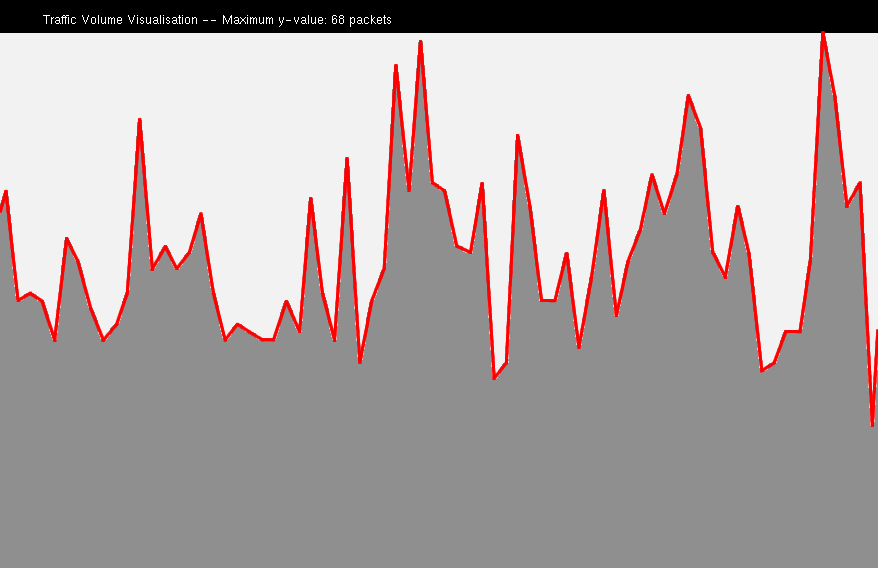
\includegraphics[width=\textwidth,keepaspectratio]{img/ex0.png}

    \end{frame}

    \begin{frame}{A better visualisation}

        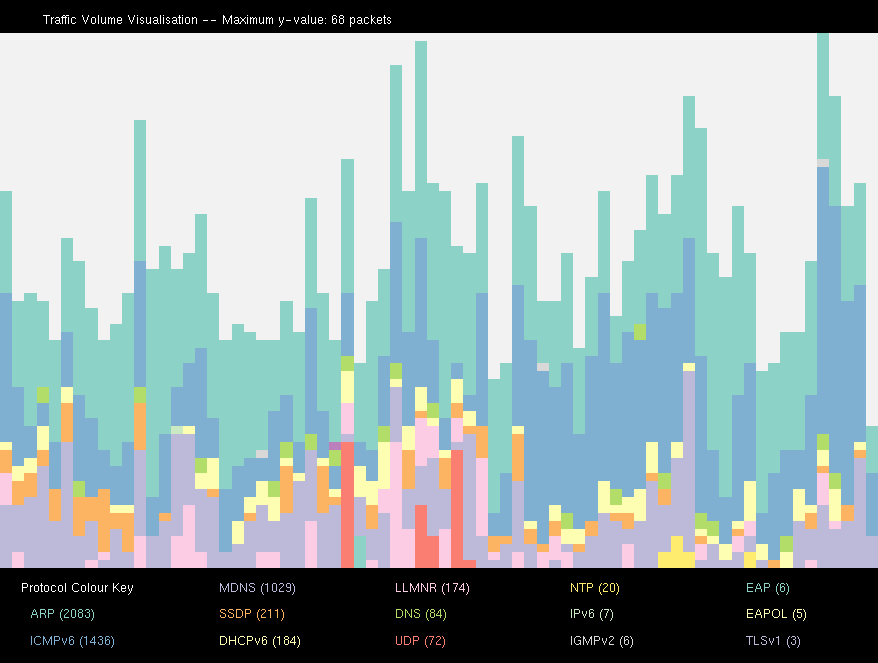
\includegraphics[width=\textwidth,keepaspectratio]{img/ex1.png}

    \end{frame}

    \begin{frame}{Teamwork}

        Tools used to encourage Synergy\small{\texttrademark} between team members
        \begin{itemize}
            \item{Version control, code hosting: \textbf{GitHub}}
            \item{Distribution of tasks: \textbf{Google Drive}, \textbf{GitHub}}
            \item{Meeting planning: \textbf{Facebook}, \textbf{Doodle}}
            \item{Shouting at people: \textbf{Facebook}, \textbf{GitHub}}
        \end{itemize}

    \end{frame} 

\end{document}
